\chapter{Utilizzo Web App}
\label{app:a}
In questo appendice verrà mostrato, attraverso brevi descrizioni e immagini, il funzionamento  dell'applicazione. I dati mostrati sono inventati e hanno il solo scopo di simulare l'utilizzo da parte di un utente della \textit{Web Application}.

\section{Accesso all'applicazione}

Una volta digitato l'indirizzo dell'applicazione, l'utente verrà accolto dalla seguente schermata, dove potrà effettuare l'accesso all'applicazione.

\begin{figure}
\begin{center}
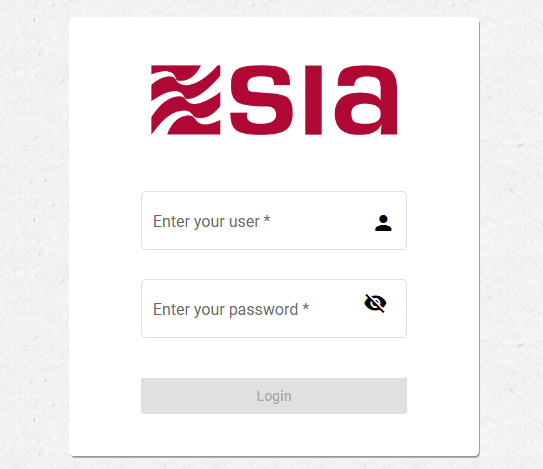
\includegraphics[width=0.7\columnwidth]{images/login1.png}
\end{center}
\caption{Pagina di login dell'applicazione}
\label{fig:login}
\end{figure}


Effettuato l'accesso l'utente sarà indirizzato verso la pagina principale, visibile in \ref{fig:home}.

\begin{figure}
\begin{center}
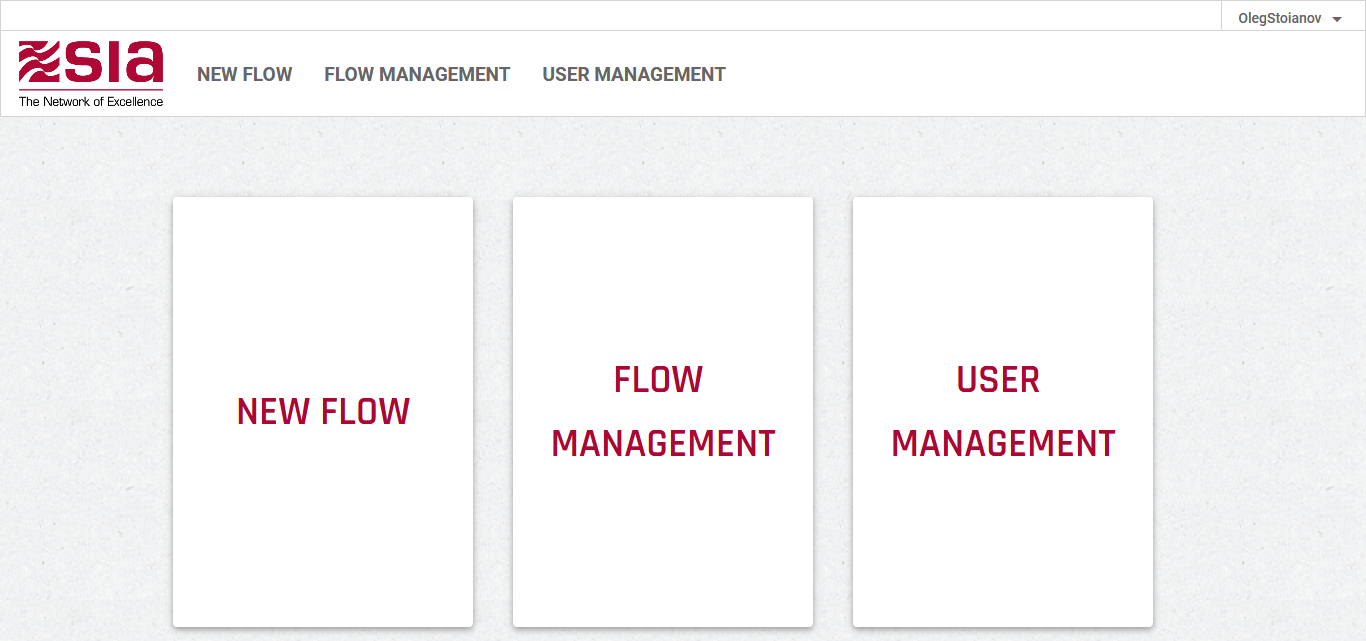
\includegraphics[width=1.0\columnwidth]{images/home.png}
\end{center}
\caption{Pagina principale dell'applicazione}
\label{fig:home}
\end{figure}


\section{Creazione nuovo flusso}

% \subsection{Fase di \textit{retrieve}}
L'utente una volta recatosi nella sezione per la creazione di un nuovo flusso, visualizza inzialmente la seguente schermata.


\begin{figure}
\begin{center}
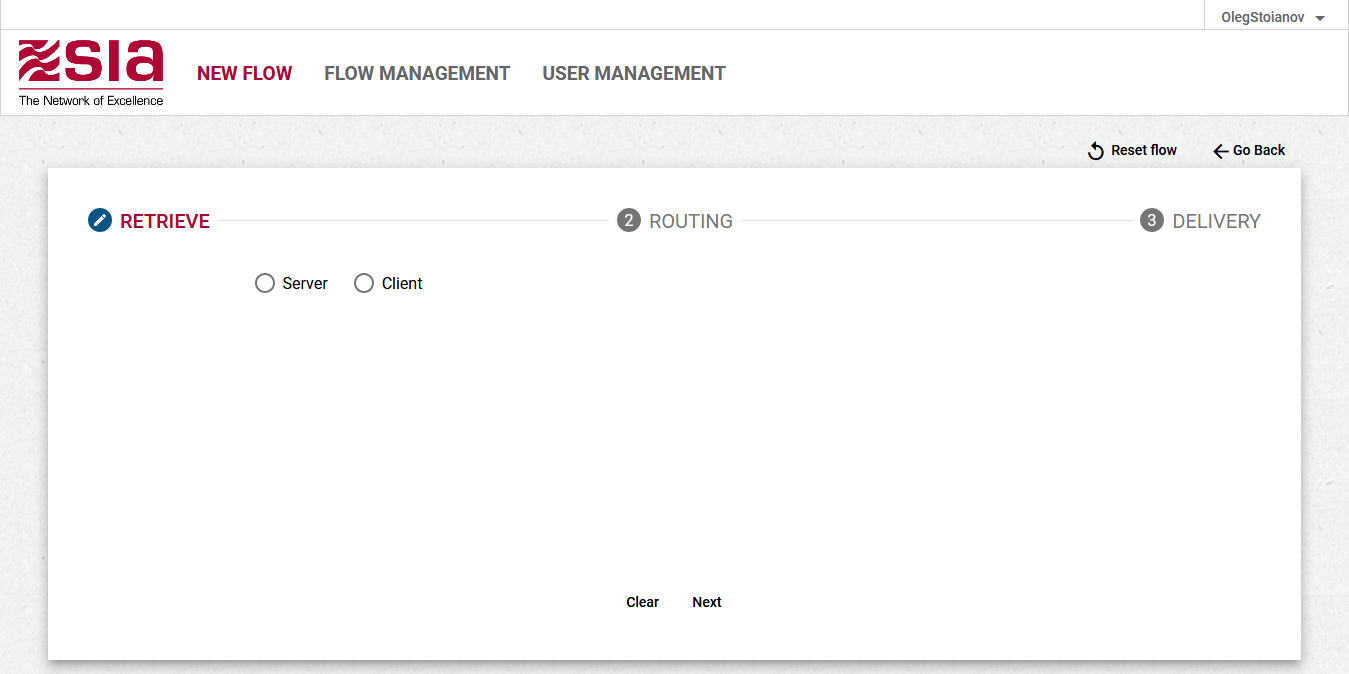
\includegraphics[width=1.0\columnwidth]{images/retrieve11.png}
\end{center}
\caption{Pagina di retrieve}
\label{fig:retrieve1}
\end{figure}
\clearpage


L'utente seleziona \textit{client} se il file dev'essere recuperato dal sistema oppure \textit{server} se il file viene inviato al sistema.
In ambedue i casi compila le informazioni richieste.

\begin{figure}
\begin{center}
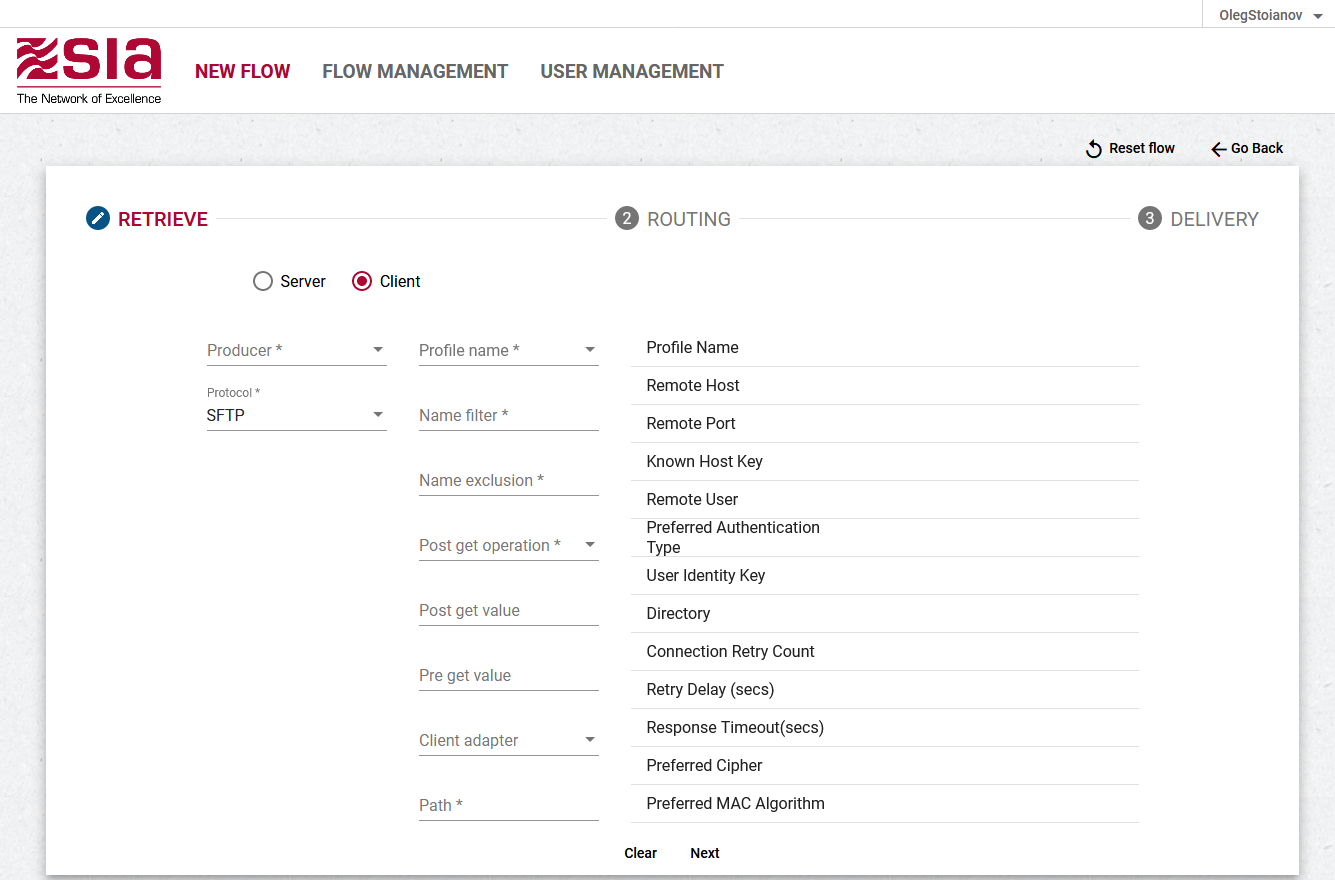
\includegraphics[width=1.0\columnwidth]{images/retrieve3.png}
\end{center}
\caption{Parametri recupero file SFTP}
\label{fig:cli}
\end{figure}


\begin{figure}
\begin{center}
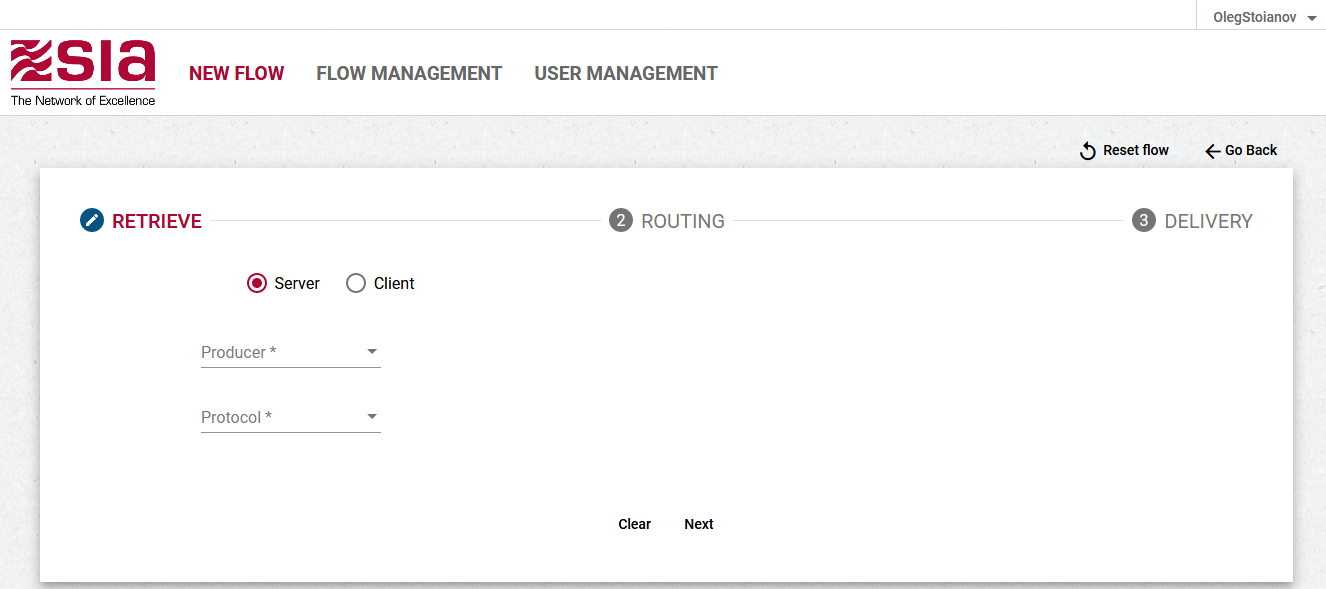
\includegraphics[width=1.0\columnwidth]{images/retrieve22.png}
\end{center}
\caption{Parametri ricezione file}
\label{fig:ser}
\end{figure}



\clearpage


Compilati i parametri per la fase di \textit{retrieve}, l'utente deve compilare quelli successivi della \textit{routing}.


\begin{figure}
\begin{center}
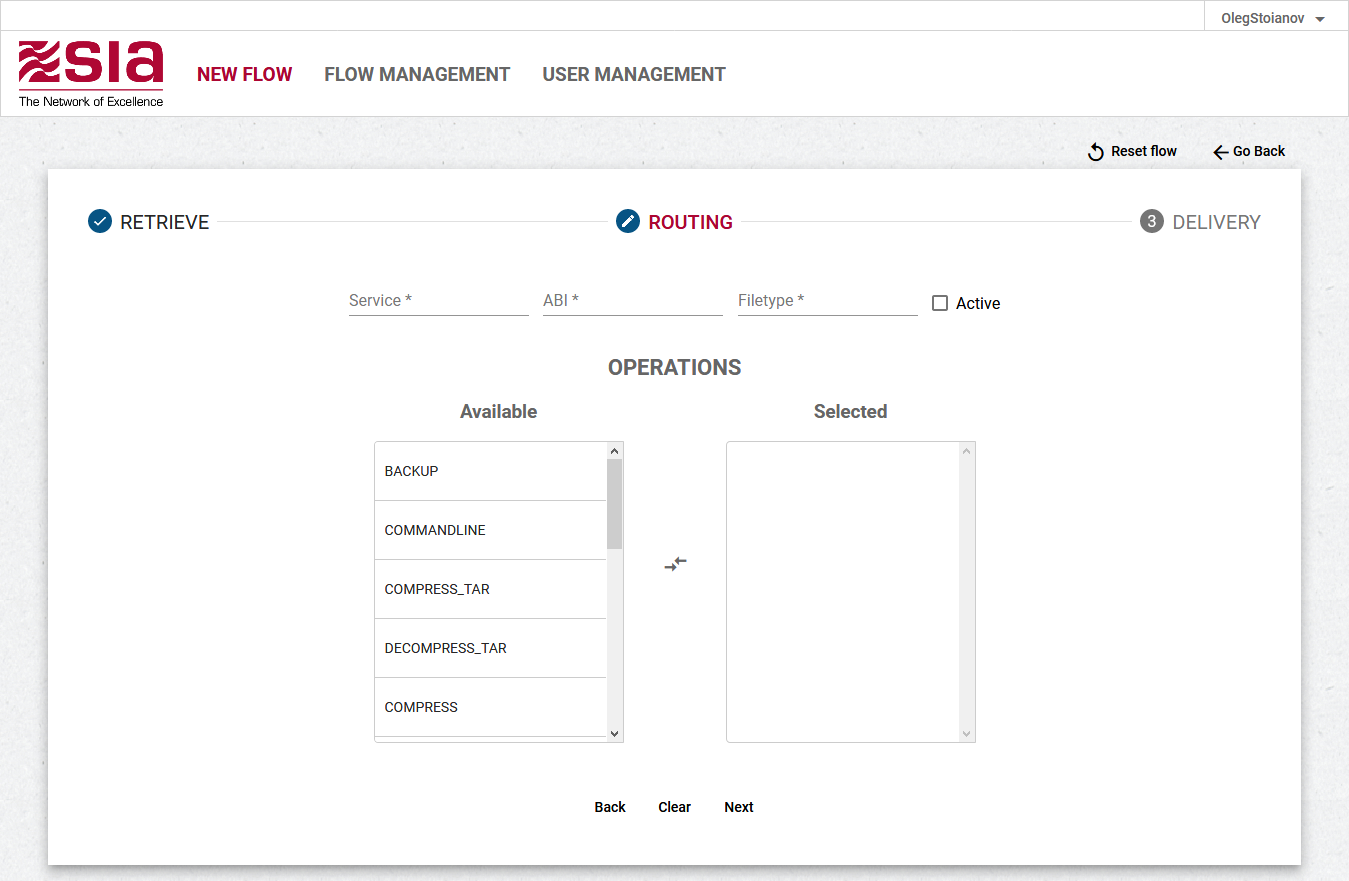
\includegraphics[width=1.0\columnwidth]{images/routing1.png}
\end{center}
\caption{Parametri identificazione flusso}
\label{fig:routing1}
\end{figure}

L'utente trascina le tipolgie di operazioni che vuole siano effettuate durante questa fase per il flusso.

\begin{figure}
\begin{center}
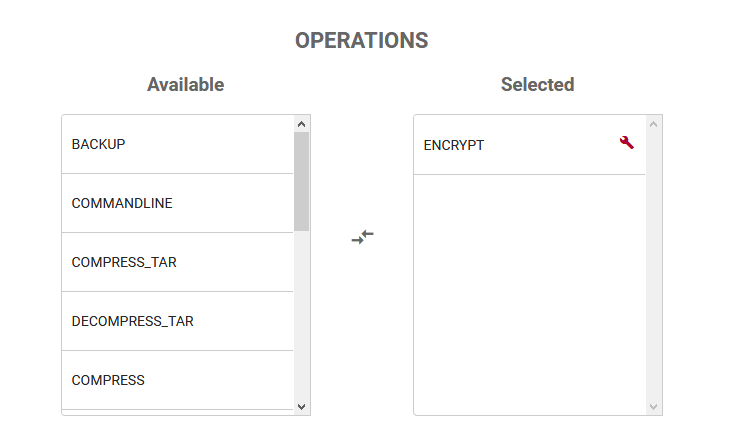
\includegraphics[width=0.6\columnwidth]{images/ope.png}
\end{center}
\caption{Operazione selezionabili}
\label{fig:ope}
\end{figure}

Cliccando sulla chiave inglese di una determinata tipologia di operazione, visibile nella figura \ref{fig:ope}, è possibile selezionare un'operazione esistente oppure crearne una ex novo.


\begin{figure}
\begin{center}
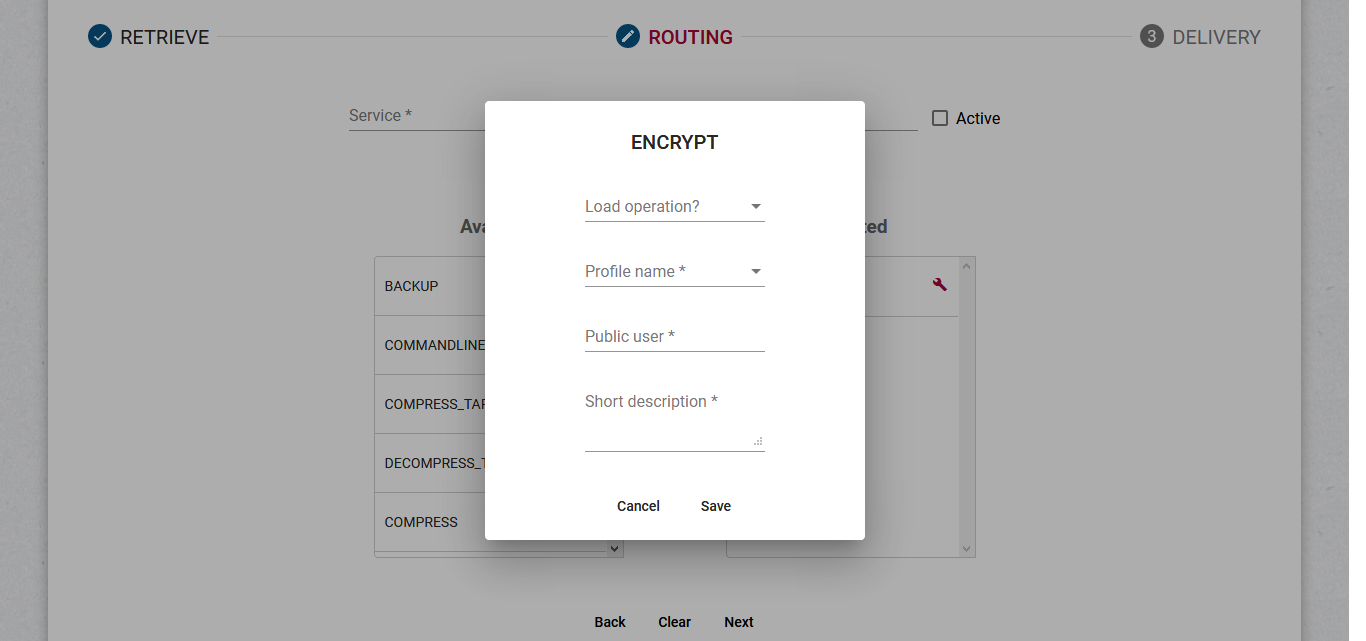
\includegraphics[width=1.0\columnwidth]{images/ope1.png}
\end{center}
\caption{Modifica o utilizzo operazione}
\label{fig:ope1}
\end{figure}

Infine l'utente seleziona il destinatario del flusso, visualizzando le informazioni riguardanti ad esso recuperate dal sistema.

\begin{figure}
\begin{center}
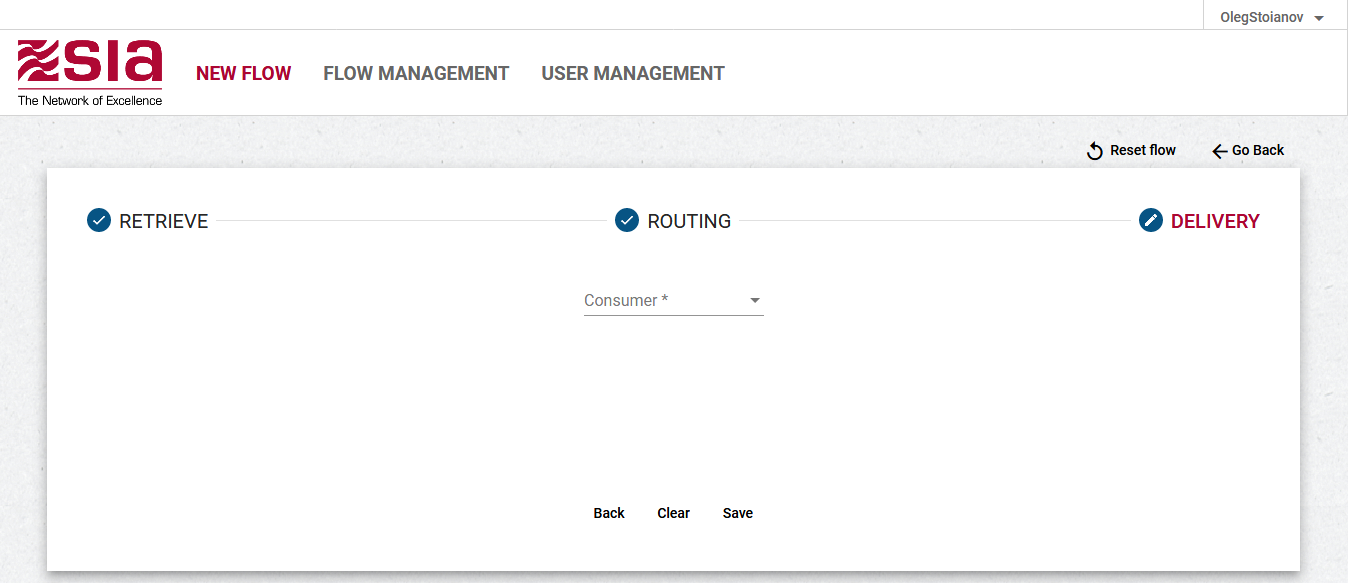
\includegraphics[width=1.0\columnwidth]{images/delive.png}
\end{center}
\caption{Selezione destinatario}
\label{fig:deli}
\end{figure}

Per salvare correttamente il flusso creato l'utente deve premere con il cursore sul bottone \textit{Save}, visibile nella parte bassa della figura \ref{fig:deli}.

\clearpage
\section{Gestione flussi esistenti}
 L'utente visitando la sezione riguardante la gestione dei flussi esitenti, visualizza la schermata sottostante: 
 
%  \ref{fig:flow}

\begin{figure}
\begin{center}
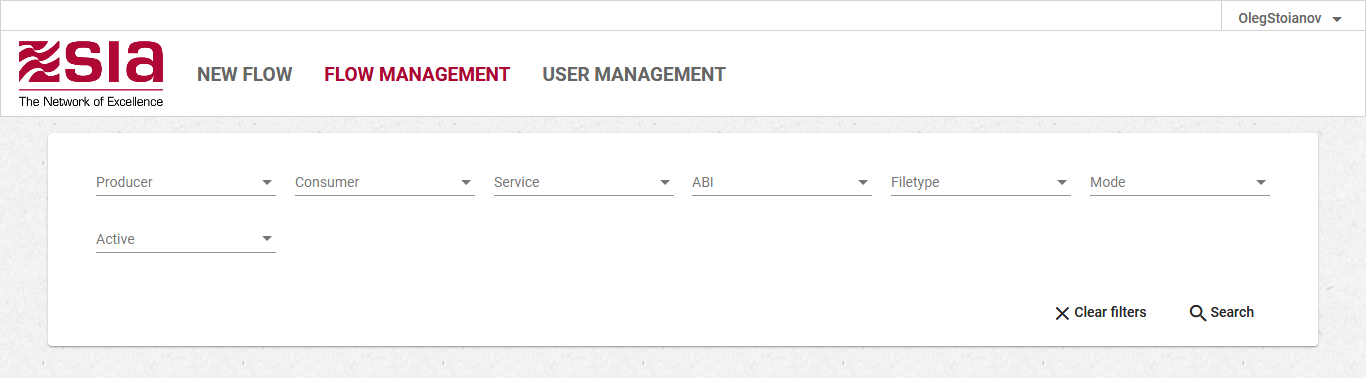
\includegraphics[width=1.0\columnwidth]{images/flow.png}
\end{center}
\caption{Sezione gestione flussi}
\label{fig:flow}
\end{figure}
\ \\
Attraverso le chiavi di ricerca, visibili in figura \ref{fig:flow} l'utente può effettuare una ricerca e visualizzare i risultati della ricerca ordinati alfabeticamente per ognuna delle chiavi.

\begin{figure}
\begin{center}
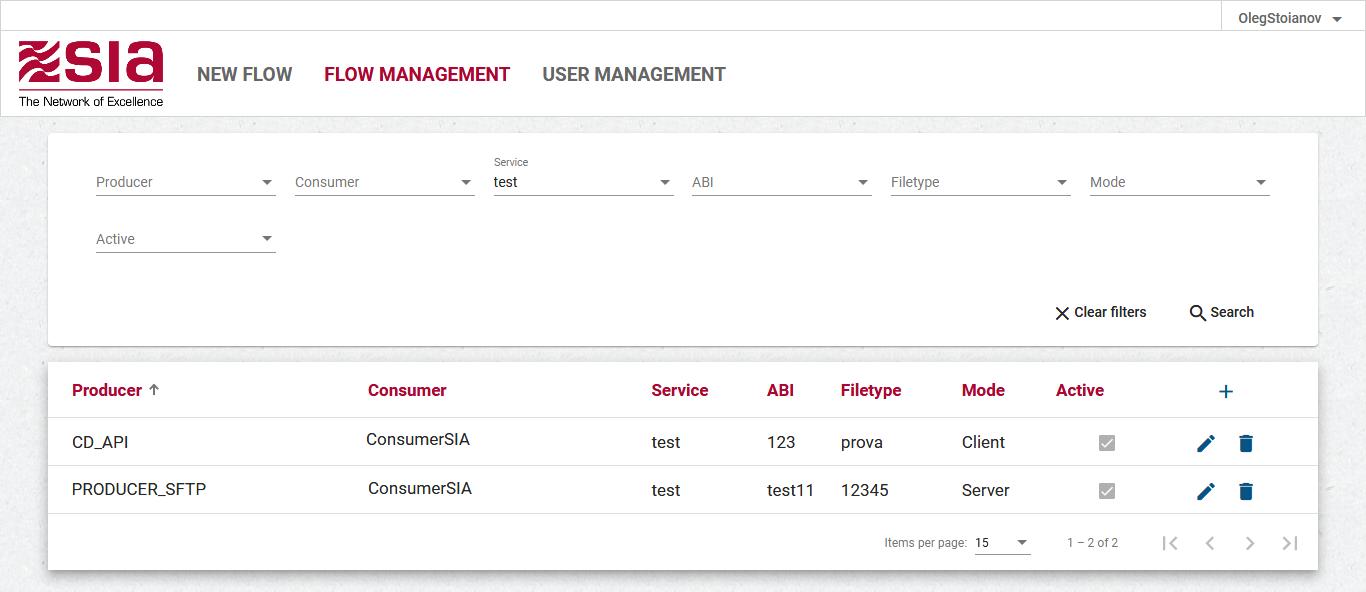
\includegraphics[width=1.0\columnwidth]{images/ricerca.png}
\end{center}
\caption{Risultato ricerca flussi}
\label{fig:ricerca}
\end{figure}

\clearpage
\ \\
Cliccando sulle apposite icone posizionate sulla destra di ogni flusso, l'utente può modificare o eliminare tale flusso. Di seguito la schermata che viene visualizzata relativa all'eliminazione.

\begin{figure}
\begin{center}
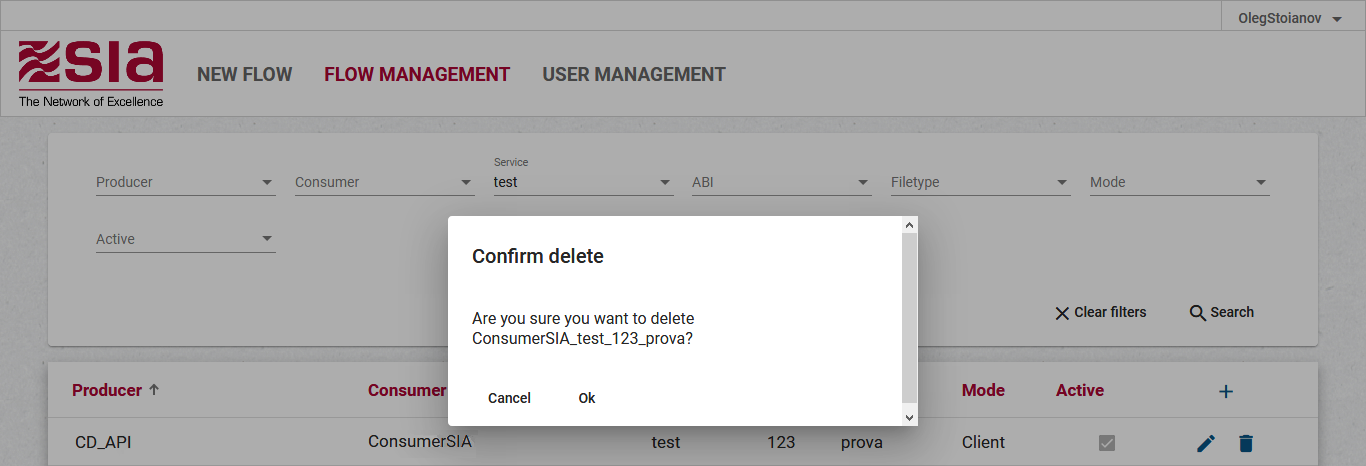
\includegraphics[width=1.0\columnwidth]{images/delete.png}
\end{center}
\caption{Eliminazione flusso}
\label{fig:delete}
\end{figure}

\section{Gestione utenti}

L'amministratore può gestire le utenze attraverso la sezione dedicata. Come visibile in figura \ref{fig:users} anche per quanto riguarda la gestione delle utenze è presente la possibilità di modificarle o eliminarle, cliccando sulle apposite icone posizionate sulla destra.



\begin{figure}
\begin{center}
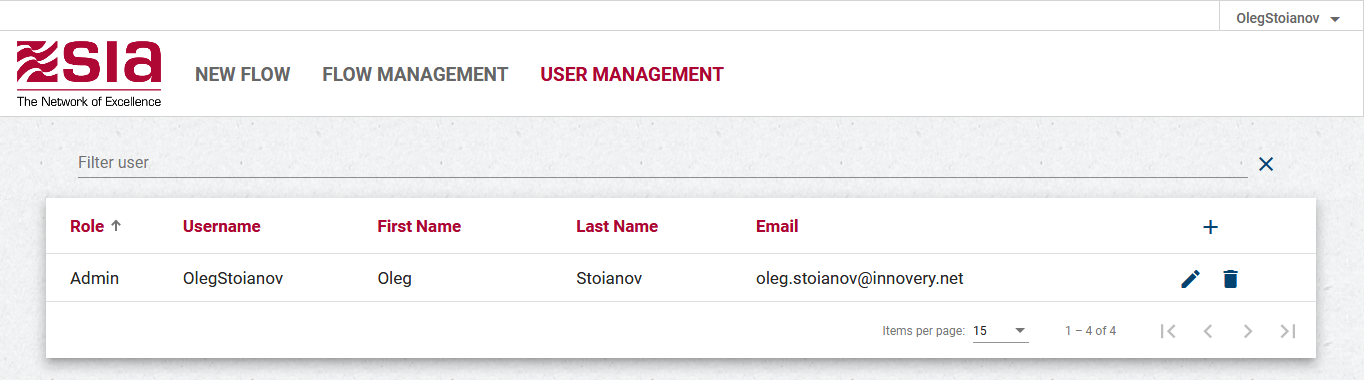
\includegraphics[width=1.0\columnwidth]{images/users.png}
\end{center}
\caption{Gestione utenze}
\label{fig:users}
\end{figure}
